\documentclass[addpoints]{exam}
\usepackage[utf8]{inputenc}
\usepackage[spanish]{babel}
\usepackage[T1]{fontenc}
\usepackage{charter}
\usepackage{amsmath}
\usepackage{amsfonts}
\usepackage{amssymb}
\usepackage{graphicx}
\usepackage{tikz}
\usepackage[outline]{contour} % glow around text
\usetikzlibrary{babel,calc,patterns,decorations.pathmorphing,decorations.markings,arrows.meta,shapes.geometric}
\usetikzlibrary{calc}
\tikzset{>=latex}
\contourlength{1.1pt}
\usepackage{tikz-3dplot}
\usepackage{multicol}
\usepackage{exam-randomizechoices}
\usepackage[left=1cm,right=1cm,top=2cm,bottom=2cm]{geometry}
\usepackage[font=small,labelfont={small,bf},margin=0.5cm,justification=justified]{caption}
\usepackage[font=small,labelfont={small,bf}]{subcaption}
\usepackage[italic,defaultmathsizes]{mathastext}
\usepackage{hyperref}
\usepackage{calculator}
\usepackage[breakable]{tcolorbox}
\usepackage{multirow}
\usepackage{tabularx}
\usepackage{cancel}
\usepackage{tipa}
\usepackage{enumerate}

%\pointpoints{punto}{puntos}
%\bonuspointpoints{punto extra}{puntos extra}

\renewcommand{\solutiontitle}{\textbf{Solución: }}
\renewcommand{\thequestion}{\bfseries\arabic{question}}

\newcommand{\sgn}{\mathop{\mathrm{sgn}}}
\newcommand{\diff}[0]{\mathrm{d}}
\newcommand{\fdiff}[2]{\frac{\mathrm{d} #1}{\mathrm{d} #2}}
\newcommand{\pdiff}[2]{\frac{\partial #1}{\partial #2}}
\newcommand{\fddiff}[2]{\frac{\mathrm{d^2} #1}{\mathrm{d} #2^2}}
\newcommand{\pddiff}[2]{\frac{\partial^2 #1}{\partial {#2}^2}}
\newcommand{\grado}[0]{^{\circ}}
\newcommand{\angulo}[3]{#1\grado \, #2' \, #3''}
\newcommand{\chel}[4]{^{#1}_{#2}\mbox{#3}^{#4}}
\newcommand{\valmed}[1]{\left\langle #1 \right\rangle}
\newcommand{\E}[1]{\times 10^{#1}}
\newcommand{\ver}[1]{\hat{\vec{#1}}}
\newcommand{\vecg}[1]{\boldsymbol{#1}}
\newcommand{\iu}{\mathrm{i}}
\newcommand{\norm}[1]{\left\vert\left\vert #1 \right\vert\right\vert}
\newcommand{\abs}[1]{\left\vert #1 \right\vert}
\newcommand{\tens}[1]{\mathbb{#1}}
\newcommand{\rr}{\mathbb{R}}
\newcommand{\un}[1]{\text{#1}}
\newcommand{\logoUNAHUR}{
\includegraphics[scale=0.35]{/home/shluna/Proyectos/Clases_Fisica_III/imgs/logo_unahur.png }}
\renewcommand{\arraystretch}{1.5}
\newcommand{\rta}{\textbf{Respuesta: }}
\newcommand{\rtas}{\textbf{Respuestas: }}
\newcommand{\ang}{110}
\newcommand{\angu}{-30}
\newcommand{\rad}{4}
\newcommand{\mg}{1}
\newcommand{\muc}{0.5}
\newcommand{\arc}[1]{{%
  \setbox9=\hbox{#1}%
  \ooalign{\resizebox{\wd9}{\height}{\texttoptiebar{\phantom{A}}}\cr#1}}}

  \colorlet{mydarkblue}{blue!40!black}
  \colorlet{myblue}{blue!30}
  \colorlet{myred}{red!65!black}
  \colorlet{vcol}{green!45!black}
  \colorlet{watercol}{blue!80!cyan!10!white}
  \colorlet{darkwatercol}{blue!80!cyan!80!black!30!white}
  \tikzstyle{water}=[draw=mydarkblue,top color=watercol!90,bottom color=watercol!90!black,middle color=watercol!50,shading angle=0]
  \tikzstyle{horizontal water}=[water,
    top color=watercol!90!black!90,bottom color=watercol!90!black!90,middle color=watercol!80,shading angle=0]
  \tikzstyle{dark water}=[draw=blue!20!black,top color=darkwatercol,bottom color=darkwatercol!80!black,middle color=darkwatercol!40,shading angle=0]
  \tikzstyle{vvec}=[->,very thick,vcol,line cap=round]
  \tikzstyle{force}=[->,myred,very thick,line cap=round]
  \tikzstyle{width}=[{Latex[length=3,width=3]}-{Latex[length=3,width=3]}]

\hypersetup{
%      draft,
   linktocpage=true,
    colorlinks=true,
    linkcolor=blue,
    citecolor=blue,
    filecolor=blue,      
    urlcolor=blue
}

\printanswers
\qformat{\textbf{Ejercicio \thequestion}\hfill}

\pagestyle{headandfoot}
\firstpageheader{Instituto de Tecnología e Ingeniería}{\logoUNAHUR}{Física III}
\firstpageheadrule
\runningheader{Primer parcial}{\logoUNAHUR}{Física III}
\runningheadrule
\firstpagefooter{}{Página \thepage\ de \numpages}{}
\firstpagefootrule
\runningfooter{}{Página \thepage\ de \numpages}{}
\runningfootrule

\begin{document}

\renewcommand{\tablename}{Tabla}

\tdplotsetmaincoords{70}{110}

\begin{tcolorbox}[colback=white,arc=0mm,colframe=black]
    \begin{center}
        \Large\textbf{Física III -- Primer parcial}
    \end{center}
\end{tcolorbox}

\vspace{11pt}

\begin{questions}

    \question Un móvil recorre una pista circular peraltada cierto angulo $\varphi$, tal como se muestra en la Figura~\ref{fig:peralte}, y que tiene radio $R$. \\
    \begin{minipage}[c]{0.6\textwidth}
        \begin{parts}
            \part Demostrar que la rapidez con la que el móvil debe recorrer la pista para describir un movimiento circular uniforme debe ser $$ v = \sqrt{g \, R \, \tan \varphi}$$
            \part Demostrar que el periodo del movimiento viene dado por $$ P = 2 \, \pi \sqrt{\frac{R}{g \tan \varphi}} $$
            \part ¿Cuál es la fuerza que obliga al móvil a describir la trayectoria circular?
            \part ¿Es constante la velocidad del móvil? Justifique su respuesta.
        \end{parts}
    \end{minipage}
    \hfill
    \begin{minipage}[c]{0.3\textwidth}
        \begin{center}
            \begin{tikzpicture}[scale=1]
                \node[inner sep=0pt] at (0,0) {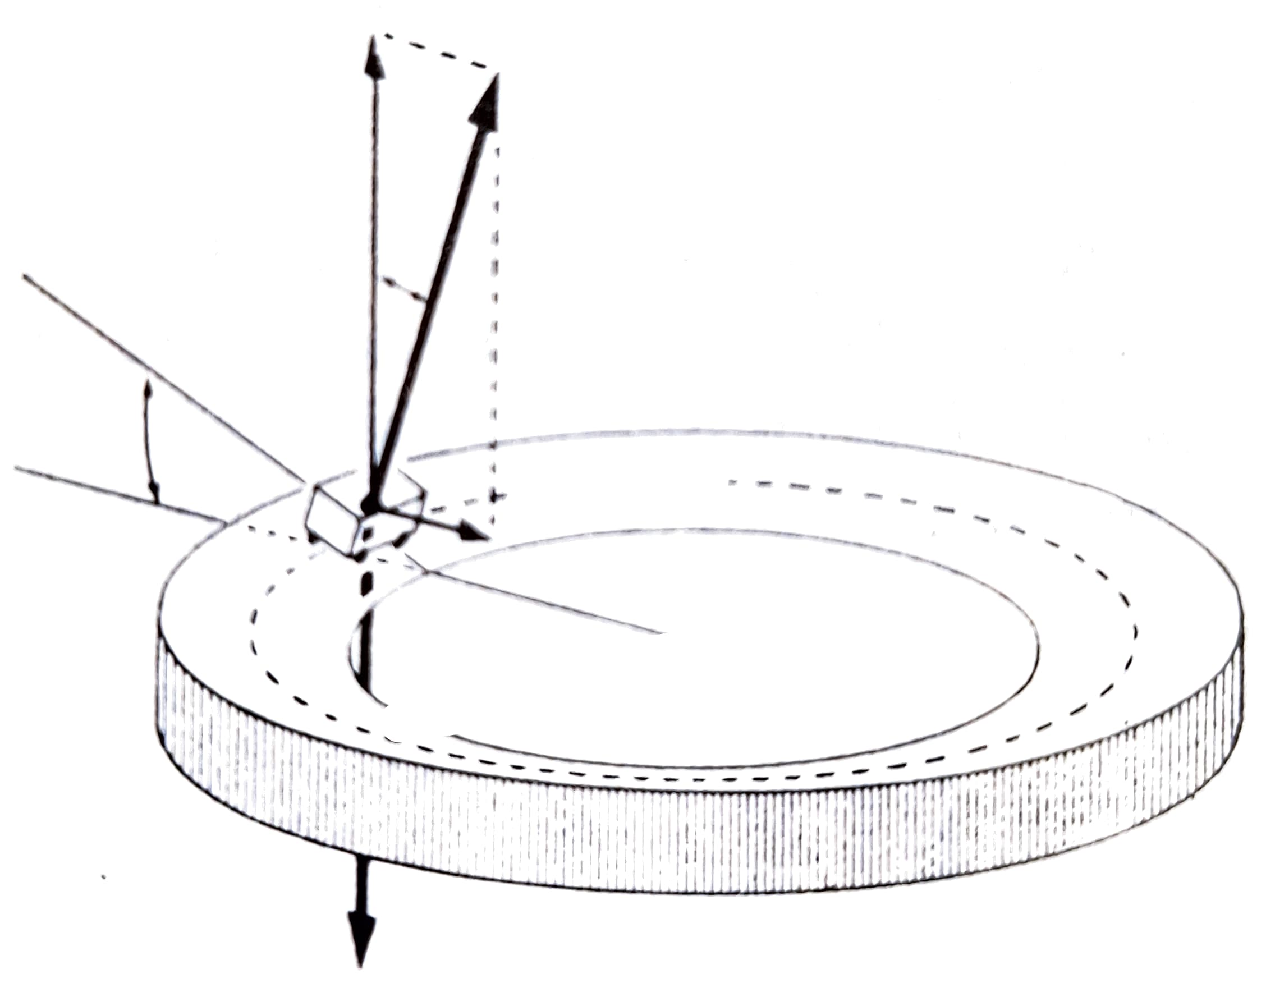
\includegraphics[width=\textwidth]{/home/shluna/Proyectos/Clases_Fisica/figs/peralte.pdf}};
                \node at (-0.25,-0.3) {$R$};
                \node at (-0.4,2.25) {$\vec{F}_\text{N}$};
                \node at (-1.3,-2.5) {$\vec{F}_\text{g}$};
                \node at (-1.05,1.2) {$\varphi$};
                \node at (-2.5,0.3) {$\varphi$};
            \end{tikzpicture}
            \captionof{figure}{ }
            \label{fig:peralte}
        \end{center}
    \end{minipage}
    
    \question \label{ej:bloque_plano_MCU} Un bloque de masa $m$ está atado a un clavo situado en el centro de una superficie horizontal sin rozamiento. Se desprecia también el efecto de cualquier otra fuerza externa, como la resistencia del aire. El hilo que une el bloque con el clavo está totalmente estirado y tiene una longitud $R$. El bloque se encuentra inicialmente en reposo, pero en cierto instante se aplica sobre el bloque una fuerza de módulo constante ($F$) y cuya dirección es siempre tangente a la trayectoria, tal como se muestra en la Figura~\ref{fig:plano_bloque_MCU}. \label{ej:plano_bloque_MCU}
    
    \begin{minipage}[c]{0.4\textwidth}
        \begin{parts}
            \part Si el módulo de la tensión del hilo puede alcanzar un valor máximo $F_{T,\text{max}}$ sin romperse, demostrar que el tiempo que transcurre desde que el bloque empieza a moverse hasta que el módulo de la tensión alcanza dicho valor máximo viene dado por $$ \Delta t = \frac{1}{F} \sqrt{m \, F_{T,\text{max}} \, R} $$
            \part Mostrar también que el desplazamiento angular del bloque en el intervalo de tiempo calculado en el apartado anterior es $$ \Delta \theta = \frac{F_{T,\text{max}}}{2 \, F}$$
        \end{parts}
    \end{minipage}
    \hfill
    \begin{minipage}[c]{0.55\textwidth}
        \begin{center}
            \begin{tikzpicture}[scale=1,tdplot_main_coords]
                \draw[thick] (-4,-4,0) -- (4,-4,0) -- (4,4,0) -- (-4,4,0) -- cycle;
                \draw[dashed] (0,0,0) circle (3);
                \draw[fill=gray!40] (0,0,0) circle (0.1);
                \draw[fill=gray!40] ({0.1*cos(\ang)},{0.1*sin(\ang)},0) -- ({0.1*cos(\ang)},{0.1*sin(\ang)},0.5) -- ({-0.1*cos(\ang)},{-0.1*sin(\ang)},0.5) -- ({-0.1*cos(\ang)},{-0.1*sin(\ang)},0);
                \draw[fill=gray!40] (0,0,0.5) circle (0.1);
                \draw[thick] (0,-0.1,0.25) arc (-90:90:0.1);
                \draw[thick] (0,0.1,0.25) -- node[anchor=south]{$R$} (0,3,0.25);
                %\draw[thick,-Kite] (4,3,0.25) -- (3.6,3,0.25);
                %\draw[thick,red,-latex] (0,3,0.25) -- node[anchor=north west]{$\vec{v}_{\text{B}2}$} (-3,3,0.25);
                \draw[thick,-latex] (0,3,0.25) -- (-3,3,0.25) node[anchor=north west]{$\vec{F}$};
                % \draw[densely dashed] (-3,3,0.25) -- (-5,3,0.25);
                % \draw[thick,-Kite] (-5,3,0.25) -- (-5.25,3,0.25);
                % \draw[thick,-latex,blue] (-4,3.5,0.25) -- node[anchor=north west]{$\vec{v}_{\text{A}2}$} (-5.5,3.5,0.25);
                \draw[fill=gray!40] (-0.5,2.75,0) -- (-0.5,3.25,0) -- (0.5,3.25,0) -- (0.5,2.75,0) -- cycle;
                \draw[fill=gray!40] (-0.5,2.75,0.5) -- (-0.5,3.25,0.5) -- (0.5,3.25,0.5) -- (0.5,2.75,0.5) -- cycle;
                \draw[fill=gray!40] (0.5,2.75,0) -- (0.5,2.75,0.5) -- (0.5,3.25,0.5) -- (0.5,3.25,0) -- cycle;
                \draw[fill=gray!40] (0.5,3.25,0) -- (0.5,3.25,0.5) -- (-0.5,3.25,0.5) -- (-0.5,3.25,0) -- cycle;
                %\draw[densely dashed] (3.6,3,0.25) -- (0.5,3,0.25);
            \end{tikzpicture}
            \captionof{figure}{ }
            \label{fig:plano_bloque_MCU}
        \end{center}
    \end{minipage}

    \question \label{ej:OAS} Un oscilador armónico simple está formado por una masa puntual de $6$ kg y un resorte cuya constante es $2400\, \frac{\text{N}}{\text{m}}$, tal como se muestra en la Figura~\ref{fig:OAS_v0pos} (\subref{fig:oas_reposo_v0pos}). Se le imprime a la masa puntual una velocidad inicial $\vec{v}_0 = \left(-6\, \frac{\text{m}}{\text{s}};0\right)$, tal como se muestra en la Figura~\ref{fig:OAS_v0pos} (\subref{fig:oas_inicial_v0pos}).

    \begin{figure}[h]
        \centering
        \begin{subfigure}{0.45\textwidth}
            \centering
            \begin{tikzpicture}[scale=1.75]
                \draw[decoration={coil,segment length = 2mm,amplitude = 2mm,aspect = 0.5,post length = 1mm,pre length = 1mm},decorate,thick,black!50] (0,0) -- (2,0);
                \draw[thick] (0,-0.25) -- (0,0.25);
                \node at (1,0.3) {$k$};
                \draw[-latex] (-0.5,0) -- (4,0) node[anchor=north]{$x$};
                \draw[-latex] (2,-0.5) -- (2,0.5) node[anchor=east]{$y$};
                \fill[black] (2,0) circle (0.5mm) node[anchor=south west]{$m$};
            \end{tikzpicture}
            \caption{ }
            \label{fig:oas_reposo_v0pos}
        \end{subfigure}
        \begin{subfigure}{0.45\textwidth}
            \centering
            \begin{tikzpicture}[scale=1.75]
                \draw[decoration={coil,segment length = 2mm,amplitude = 2mm,aspect = 0.5,post length = 1mm,pre length = 1mm},decorate,thick,black!50] (0,0) -- (2,0);
                \draw[thick] (0,-0.25) -- (0,0.25);
                \node at (1,0.3) {$k$};
                \draw[-latex] (-0.5,0) -- (4,0) node[anchor=north]{$x$};
                \draw[-latex] (2,-0.5) -- (2,0.5) node[anchor=east]{$y$};
                \fill[black] (2,0) circle (0.5mm) node[anchor=south west]{$m$};
                \draw[thick,-latex] (2,0.3) -- (1.5,0.3) node[anchor=south]{$\vec{v}_0$};
            \end{tikzpicture}
            \caption{ }
            \label{fig:oas_inicial_v0pos}
        \end{subfigure}
        \caption{Esquema del \ref{ej:OAS}.}
        \label{fig:OAS_v0pos}
    \end{figure}

    \begin{parts}
        \part Determinar la frecuencia angular ($\omega$), la amplitud ($A$), el periodo ($P$) y la frecuencia física ($f$) de las oscilaciones.
        \checkboxchar{$\Box$}
        \part ¿Para qué valores de la elongación la rapidez de la masa puntual alcanza sus valores máximo y mínimo?
        \part ¿Para qué valores de la elongación la rapidez de la masa puntual se anula?
        \part ¿Para qué valores de la elongación componente $x$ de la aceleración impresa a la masa puntual alcanza sus valores máximo y mínimos?
        \part ¿Para qué valores de la elongación la componente $x$ de la aceleración impresa a la masa puntual se anula?
        \part Si se duplica la rapidez inicial, ¿se modifican los valores de $P$, $f$ y $\omega$? ¿Por qué?
        \part Si la velocidad inicial fuese , $\vec{v}_0 = \left(6\, \frac{\text{m}}{\text{s}};0\right)$ ¿se modifican los valores de $A$, $P$, $f$ y $\omega$? ¿Por qué?
    \end{parts}

    \question \label{ej:equilbrio_CR} Una barra rígida que tiene una longitud de 3 m está unida a dos bloques mediante alambres inextensibles y de masa despreciable. El alambre que une la barra con el bloque $A$ pasa por una polea sin rozamiento y de masa también despreciable. Por otro lado, el segmento que va entre el extremo derecho de la barra y la polea forma un ángulo $\psi$ con la horizontal tal que $\cos \psi = \frac{3}{5}$ y $\sen \psi = \frac{4}{5}$. El bloque $A$ tiene una masa de 2 kg y el bloque $B$ tiene una masa de 12 kg, mientras que la barra tiene 10 kg de masa. Hallar la fuerza $\vec{F}$ y las coordenadas del punto de la barra en el que debe aplicarse esta fuerza para mantener la misma en equilibrio estático en la posición que se muestra en la Figura~\ref{fig:barra}. Puede informar las componentes $x$ e $y$ de la fuerza o bien su módulo y el ángulo que forma con los $x$ positivos ($\varphi$). Suponga que la fuerza $\vec{F}$ debe colocarse en el punto $(x_F; 0)$, donde debe determinar el valor de $x_F$.

    \textbf{Pista:} La polea solamente cambia la dirección de la tensión del alambre.

    \begin{figure}[ht]
        \centering
        \begin{tikzpicture}[scale=1]
            \draw[thick,-latex] (-5,0) -- (2,0) node[anchor=north]{$x$};
            \draw[thick,-latex] (0,-2) -- (0,2) node[anchor=east]{$y$};
            \fill[black] (0,0) circle (0.3mm);
            \draw[thick] (0,0) -- (60:2);
            \draw[thick] ({2*cos(60)+0.2*cos(30)},{2*sin(60)-0.2*sin(30)}) circle (0.2cm);
            \draw[thick] ({2*cos(60)+0.2*cos(30)+0.2},{2*sin(60)-0.2*sin(30)}) -- ({2*cos(60)+0.4*cos(30)},-0.5);
            \fill[black] ({2*cos(60)+0.2*cos(30)},{2*sin(60)-0.2*sin(30)}) circle (0.3mm);
            \draw (0.5,0) arc (0:60:0.5);
            \draw[thick,fill=gray!40!white] ({2*cos(60)+0.4*cos(30)-0.25},-0.5) rectangle ({2*cos(60)+0.4*cos(30)+0.25},-1);
            \node at ({2*cos(60)+0.2*cos(30)+0.2},-0.75) {$A$};
            \node at (30:0.7) {$\psi$};
            \draw[thick] (-4,0) -- (-4,-0.5);
            \draw[thick,fill=gray!40!white] (-4.3,-0.5) rectangle (-3.7,-1.1);
            \node at (-4,-0.8) {$B$};
            \draw[latex-latex] (-4,1) -- node[fill=white]{$L$} (0,1);
            \draw (-4,0.8) -- (-4,1.2);
            \draw[latex-latex] (-2,0.5) -- node[fill=white]{$\frac{L}{2}$} (0,0.5);
            \draw (-2,0.4) -- (-2,0.6);
            \draw[latex-latex,red] (-3,-0.5) -- node[fill=white]{$x_F$} (0,-0.5);
            \draw[red] (-3,-0.3) -- (-3,-0.7);
            \draw[fill=gray!40!white,thick] (-4,-0.1) rectangle (0,0.1);
            \begin{scope}[shift={(-3,0)}]
                \draw[thick,-latex,red] (0,0) -- (120:2) node[anchor=east]{$\vec{F}$};
                \fill[red] (0,0) circle (0.3mm);
                \draw[red] (0.5,0) arc (0:120:0.5);
                \node[red] at (60:0.7) {$\varphi$};
                \draw[red] (0,0) -- (0.75,0);
            \end{scope}
            \fill[black] (-2,0) circle (0.4mm) node[anchor=south,yshift=0.3]{\textsc{cm}}; 
        \end{tikzpicture}
        \caption{Esquema del \ref{ej:equilbrio_CR}. Se indica el centro de masa de la barra (\textsc{cm}).}
        \label{fig:barra}
    \end{figure}

    \question Un bloque de 8 kg de masa se encuentra en reposo sobre una superficie horizontal lisa. Una cuerda inextensible atada al bloque pasa por una polea, cuyo diámetro tiene 15 cm, y en el otro extremo de la cuerda cuelga otro bloque cuya masa es también de 8 kg, tal como se muestra en la Figura~\ref{fig:vinculados2}. Se abandona el sistema desde el reposo y se observa que el bloque recorre 5 m en 2 s.
    \begin{parts}
        \part ¿Cuál es el momento de inercia de la polea?
        \part ¿Cuál es la tensión en cada parte de la cuerda?
    \end{parts}

    \begin{figure}[h]
        \centering
        \begin{tikzpicture}[scale=1]
            \fill[pattern=north east lines] (-5,-0.25) -- (-0.5,-0.25) -- (-0.5,-3.5) -- (-0.7,-3.5) -- (-0.7,-0.45) -- (-5,-0.45) -- cycle;
            \draw (0,0) circle (0.25cm);
            \draw (-3,0.25) -- (0,0.25);
            \draw (0.25,0) -- (0.25,-2);
            \draw[fill=gray!40] (-3,-0.25) -- (-3,0.75) -- (-4,0.75) -- (-4,-0.25) -- cycle;
            \draw[fill=gray!40] (0,-2) -- (0.5,-2) -- (0.5,-2.5) -- (0,-2.5) -- cycle;
            \draw[thick] (-5,-0.25) -- (-0.5,-0.25) -- (-0.5,-3.5);
            \node at (-3.5,0.25) {$A$};
            \node at (0.25,-2.25) {$B$};
            \draw[thick] (-0.5,-0.25) -- (0,0);
            \draw[fill=black] (0,0) circle (0.5mm);
        \end{tikzpicture}
        \caption{ }
        \label{fig:vinculados2}
    \end{figure}

\end{questions}

\end{document}